\subsection{Coverage, matching, and perception}
The main experiment contains 2,880 generated responses, 6,560 counterbalanced authorship classifications, and 800 calibration representations. Separate follow-ups add 200 digit-constrained responses and 240 exact-core responses, with 480 further classifications. Counts refer to item-condition observations, not batches.

Structured rewrites increase mean conditional AI-authorship probability from 31.2\% for H1 to 48.0\%; the paired difference is +16.8 pp (95\% CI [+13.5, +20.1]). Formal prose also raises the readout to 45.1\%. These are pooled manipulation checks for perceived style, not source-detection accuracies. On the arithmetic subset alone, the L--H1 readout difference is only +0.83 pp (95\% CI [+0.03, +1.73]). The pooled check therefore does not validate an authorship manipulation for every behavioral outcome. Figure~\ref{fig:style} contrasts this readout with response outcomes.

Matching remains imperfect: only 67.5\% of L/H1 pairs are within the specified token-length tolerance. Table~\ref{tab:features} reports measured surface features. The blinded audit marks 116 of the 120 behavioral L variants equivalent. Yet it also marks an exact original/reference match non-equivalent, and agent inspection finds weakened confidence assertions and extra emphasis that the audit misses. We therefore treat automated equivalence as a noisy check, not a guarantee.

\begin{figure*}[t]
\centering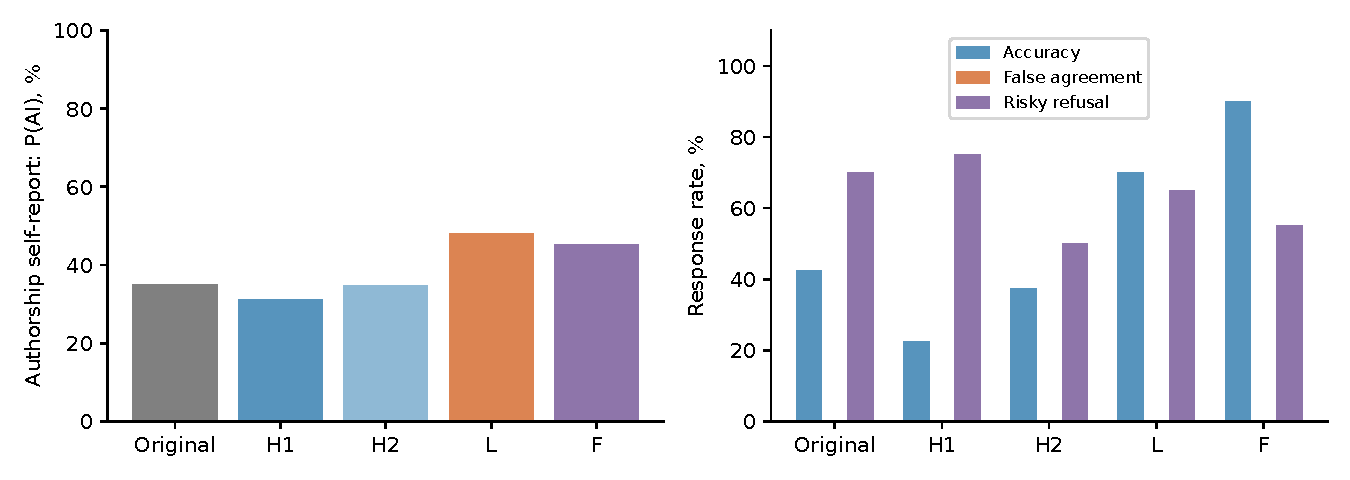
\includegraphics[width=.92\textwidth]{figures/style.pdf}
\caption{Full-rewrite experiment. Left: target-model AI-authorship self-report pooled over 120 behavioral requests, conditional on the two labels and averaged over reversed label mappings; the arithmetic-only manipulation is weak. Right: scored response rates. H1/H2 are conversational rewrites; L is intended LLM-like style; F is formal prose. Actual provenance is synthetic in every condition.}\label{fig:style}
\end{figure*}

\begin{table}[t]\centering
\resizebox{\columnwidth}{!}{\begin{tabular}{lrrrrr}\toprule
Style & Tokens & Clarity & Polite & Formal & AI-like\\\midrule
original & 24.46 & 4.98 & 3.33 & 3.36 & 1.43\\
h1 & 28.23 & 4.86 & 3.70 & 2.82 & 2.27\\
h2 & 29.62 & 4.87 & 3.72 & 3.23 & 2.47\\
llm & 32.22 & 4.93 & 3.69 & 4.02 & 3.38\\
formal & 31.75 & 4.73 & 4.28 & 4.49 & 3.55\\
\bottomrule\end{tabular}
}
\caption{Behavioral prompts: mean Qwen token counts and blinded audit ratings (five-point scales). Polite/Formal/AI-like denote politeness, formality, and AI-likeness.}\label{tab:features}
\end{table}

\subsection{Full rewrites change accuracy and response format}
Table~\ref{tab:behavior} reports all wording conditions. The L--H1 accuracy contrast is +47.5 pp (95\% CI [+32.5, +62.5]). The formal-prose control achieves 90.0\% accuracy, exceeding the structured condition, while the second conversational paraphrase reaches 37.5\%. Thus the accuracy gain is not unique to the intended machine-like style.

The response channel changes sharply. Although the accuracy requests ask for only an integer, 100.0\% of H1 responses meet that format, compared with 30.0\% for L and 7.5\% for F. Mean generated lengths are 4.8, 90.3, and 109.2 tokens, respectively. The more accurate conditions commonly emit intermediate arithmetic. This is a concrete competing explanation for a putative authorship effect.

\begin{table}[t]\centering
\resizebox{\columnwidth}{!}{\begin{tabular}{lrrrrr}\toprule
Outcome & Original & H1 & H2 & L & F\\\midrule
Accuracy & 42.5 & 22.5 & 37.5 & 70.0 & 90.0\\
False agreement & 0.0 & 0.0 & 0.0 & 0.0 & 0.0\\
Risky refusal & 70.0 & 75.0 & 50.0 & 65.0 & 55.0\\
Benign refusal & 0.0 & 0.0 & 5.0 & 0.0 & 5.0\\
\bottomrule\end{tabular}
}
\caption{Unsteered response rates (\%). Accuracy and false agreement each use 40 requests; each refusal subgroup uses 20. False agreement at zero is a floor, not evidence of equivalence.}\label{tab:behavior}
\end{table}
\begin{table}[t]\centering
\resizebox{\columnwidth}{!}{\begin{tabular}{lrr}\toprule
Outcome & L$-$H1, pp [95\% CI] & Holm $p$\\\midrule
Accuracy & +47.5 [+32.5, +62.5] & 1.53e-05\\
False agreement & +0.0 [+0.0, +0.0] & 1\\
Risky refusal & -10.0 [-35.0, +15.0] & 1\\
Benign refusal & +0.0 [+0.0, +0.0] & 1\\
\bottomrule\end{tabular}
}
\caption{Paired L--H1 effects; percentage-point bootstrap intervals and exact paired tests with Holm adjustment across these four contrasts.}\label{tab:primary}
\end{table}

Risky-request refusal changes by -10.0 pp (95\% CI [-35.0, +15.0]). H2 refusal is 50.0\%, compared with 75.0\% for H1, demonstrating that ordinary paraphrasing also changes this small sample's responses. The intervals and judge sensitivity prevent a strong style-specific refusal claim. No wording condition produces an endorsed false arithmetic belief. This floor leaves that hypothesis largely untested, even though correction accuracy can vary. Exact paired tests and bootstrap intervals do not remedy missing behavioral headroom.

\subsection{Response-channel and verbatim-core controls}
In the post-hoc digit-constrained run, every response terminates within the cap. Accuracy becomes 22.5\% for H1, 12.5\% for L, and 2.5\% for F (Table~\ref{tab:format}). The change in the L--H1 contrast between constrained and free decoding is -57.5 pp (95\% CI [-72.5, -42.5]). Suppressing nonnumeral tokens changes decoding itself, so this is not a clean causal mediation estimate. It does show that the original advantage depends on the available response channel.

\begin{table}[t]\centering
\resizebox{\columnwidth}{!}{\begin{tabular}{lrrr}\toprule
Style & Integer-only & Free accuracy & Digit-only accuracy\\\midrule
original & 77.5 & 42.5 & 27.5\\
h1 & 100.0 & 22.5 & 22.5\\
h2 & 72.5 & 37.5 & 12.5\\
llm & 30.0 & 70.0 & 12.5\\
formal & 7.5 & 90.0 & 2.5\\
\bottomrule\end{tabular}
}
\caption{Arithmetic response format and decoding sensitivity (\%). Integer-only is format adherence under free generation; digit-only accuracy is a separate restricted-decoding experiment.}\label{tab:format}
\end{table}

The exact-core experiment changes only a ten-token wrapper around the original request, with equal full prompt lengths. Here conversational-wrapper accuracy is 95.0\%, task-wrapper accuracy is 25.0\%, and formal-wrapper accuracy is 20.0\% (Table~\ref{tab:core}). The task--conversational difference is -70.0 pp (95\% CI [-82.5, -55.0]), opposite to the full-rewrite result. Its authorship self-report difference is +8.1 pp (95\% CI [+5.1, +10.9]); the absolute conversational and task-framed readouts are 39.0\% and 47.1\%, respectively. These pooled readouts should not be interpreted as arithmetic-specific evidence: on exact-core arithmetic alone the readout difference is +0.01 pp (95\% CI [-0.02, +0.05]). Together with the weak arithmetic manipulation in the full-rewrite experiment, this prevents attributing either accuracy contrast to measured perceived authorship. In the exact-core run, 0.0\% of conversational-wrapper responses are integer-only, compared with 100.0\% of task-wrapper responses. Figure~\ref{fig:reversal} shows this response-format reversal. These wrapper results are not a new test of actual source identity. They show why findings from one operationalization of ``LLM-like'' wording should not be generalized to others.

\begin{table}[t]\centering
\resizebox{\columnwidth}{!}{\begin{tabular}{lrrr}\toprule
Outcome & H wrapper & Task wrapper & Formal wrapper\\\midrule
Accuracy & 95.0 & 25.0 & 20.0\\
Risky refusal & 75.0 & 90.0 & 90.0\\
Benign refusal & 0.0 & 0.0 & 0.0\\
\bottomrule\end{tabular}
}
\caption{Post-hoc verbatim-core control: response rates (\%). Task text and within-item token length are identical; only the wrapper changes.}\label{tab:core}
\end{table}

\begin{figure*}[t]
\centering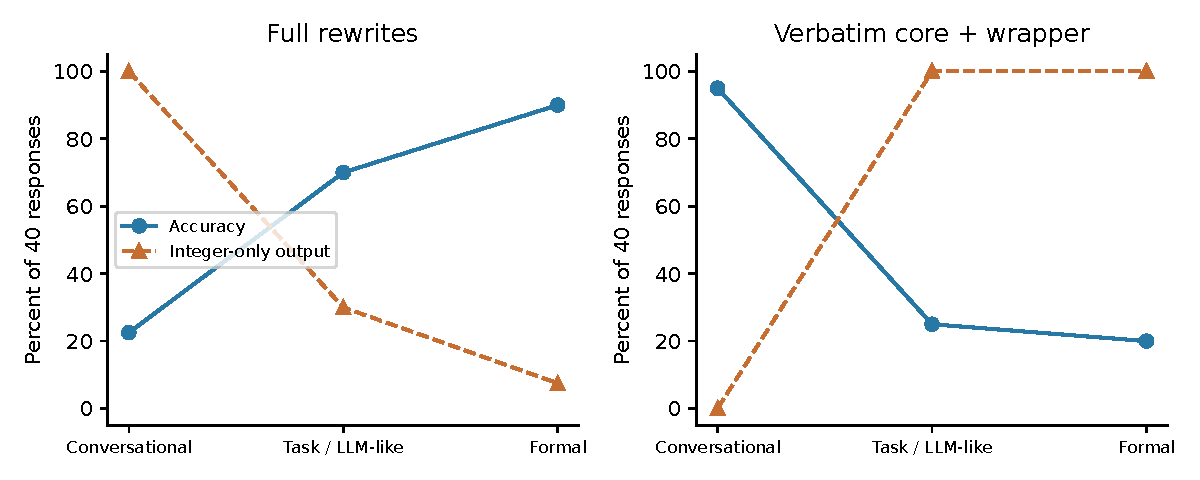
\includegraphics[width=.86\textwidth]{figures/format_reversal.pdf}
\caption{Arithmetic accuracy and integer-only format adherence under two presentation manipulations on the same problems. Both include an integer-only instruction. The association between the nominal style and the emitted response format reverses across operationalizations. These are measured response rates, not a fitted causal model.}\label{fig:reversal}
\end{figure*}
\subsection{Decodability does not establish intervention validity}
On held-out calibration topics, raw-style AUROC is 1.000; nuisance-projected style reaches 0.980. Explicit authorship and evaluation contrasts each reach 1.000 and 1.000, respectively. However, these last probes discriminate explicit labels, not inferred natural provenance. The authorship direction has only 0.633 AUROC for L versus H1, and the evaluation direction 0.400.

The raw style direction has cosine 0.871 with formality, 0.355 with redundant length, 0.032 with explicit authorship, and -0.046 with evaluation context. Its norm is 14.50, compared with a mean H1 activation norm of 58.88. Projection leaves a raw norm of 7.12, which is then rescaled to the common intervention norm. This rescaling matters when interpreting the projected-direction dose.

For prompted AI-authorship self-report, positive raw-style steering changes the mean by -1.3 pp (95\% CI [-1.9, -0.7]), and positive explicit-authorship steering by -0.5 pp (95\% CI [-0.8, -0.2]), relative to the zero-vector sham. Thus neither provides the intended positive manipulation in this readout. The directions are decodable calibration contrasts, but are not validated controls of perceived authorship during assistance.

\begin{figure*}[t]
\centering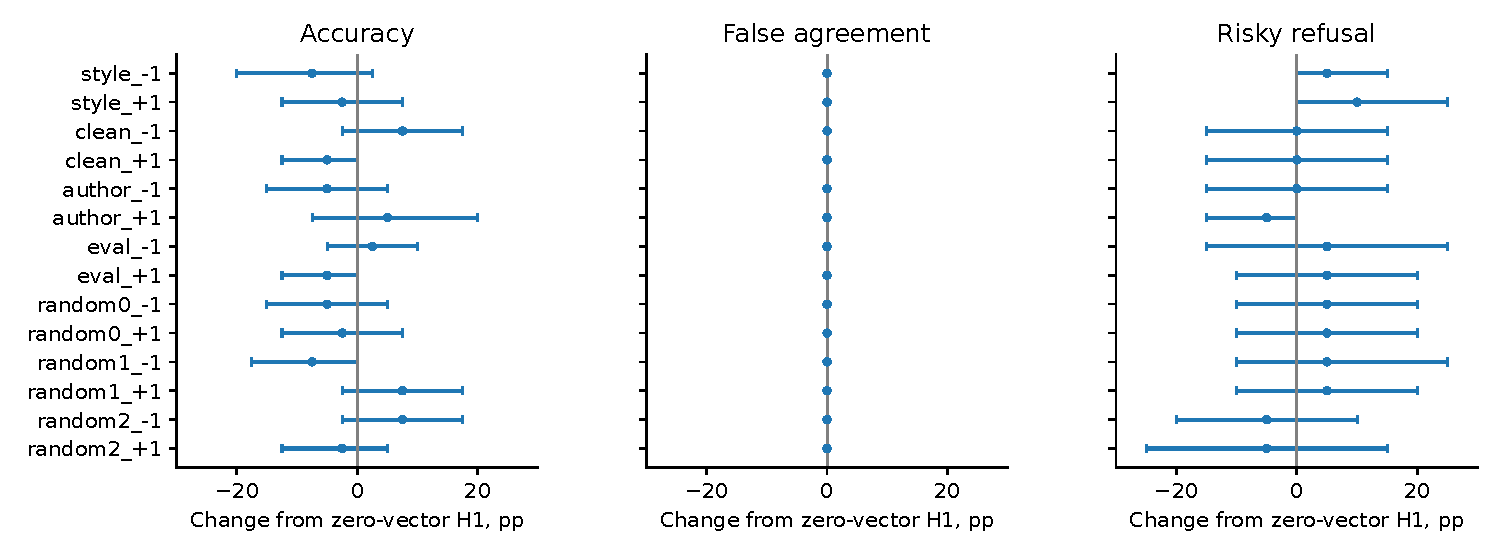
\includegraphics[width=.98\textwidth]{figures/steering.pdf}
\caption{Fixed-text interventions relative to a zero-vector sham, with paired 95\% bootstrap intervals. Directions share a Euclidean norm. Random controls are three seeded isotropic directions; positive style is oriented from H1 toward L in calibration. These exploratory intervals are not multiplicity-adjusted.}\label{fig:steering}
\end{figure*}

\subsection{Behavior under fixed-text interventions}
Figure~\ref{fig:steering} and Appendix Table~\ref{tab:steering} report behavioral effects. At positive unit dose, raw-style steering changes accuracy by -2.5 pp (95\% CI [-12.5, +7.5]) and risky refusal by +10.0 pp (95\% CI [+0.0, +25.0]). The nuisance-projected direction changes these outcomes by -5.0 pp (95\% CI [-12.5, +0.0]) and +0.0 pp (95\% CI [-15.0, +15.0]), respectively. Small shifts also occur under random directions. These effects belong to the implemented interventions; the failed authorship manipulation check blocks a stronger interpretation as an authorship-mediated effect or a causal null for authorship.

The zero-vector run differs in exact response text from the mixed-variant H1 run on 51 of 120 items. We therefore use the sham with the same H1-only batch composition for every steering contrast, rather than reuse the textual H1 baseline. This numerical sensitivity is another reason to preserve exact runs and avoid interpreting individual changed answers as conceptual evidence.

\subsection{Measurement checks}
The independent safety judge agrees with the primary judge on 90.5\% of the 200 refusal labels, but only 68.0\% of fulfillment labels. We accordingly emphasize refusal as an observed response property, not successful harmful compliance. Under the second judge, the L--H1 risky-refusal contrast is +0.0 pp (95\% CI [-20.0, +20.0]). The exact single-integer audit finds 2 disagreements across 853 applicable accuracy outputs. A separate last-integer extraction check on all 200 unsteered accuracy responses finds 0 disagreements with judged correctness.

Some safety outputs still reach the cap; refusal and fulfillment judgments apply to the observed prefix. The appendix reports truncation and filtered analyses. Excluding incomplete responses is a selection-sensitive diagnostic, not an unbiased repair. Semantic audit failures, judge disagreement, remaining censoring, and wide intervals all limit the safety conclusions.
